\documentclass{article}
\usepackage{graphicx}

\begin{document}
\title{Mirai botnet}
\author{Abhinav Narain}
\maketitle

\section{Mirai Activity and Results}
\subsection{Breakdown of Activity}
The following activity is performed by Mirai bot.
\begin{enumerate}
\item Sets up some certain data structures, and kills a previous instance is running.
\item Connects to CNC server after resolving the IP address using a DNS packet to DNS server
\item \textit{fork()} to do a SYN scan for a range of IP addresses by transmitting TCP syn frames using RAW sockets
\item Run an infinite loop waiting for SYN responses for further conducting a programmed TELNET login sequence
\item Wait for attacks from a CNC server and \textit{fork()} to launch an attack for a period of time -- one of which is a UDP flood attack conducted for 5 seconds~\ref{fig:mirai_cnc_server}
\end{enumerate}

\subsection{Expected Output of EMI}

\begin{itemize}
\item  Step 2 above should produce an EMI on spectrogram corresponding to SYN packets transmitted in bulk to certain subnets.
\item  Step 4 should show EMI on spectrogram corresponding to UDP flooding
\end{itemize}

\subsection{Lenovo laptop}
I did the experiments by running Mirai bot on the laptop.



\subsection{Raspberry Pi}
I did the experiments with Raspberry Pi as the client. As with previous experiments of UDP blasts and computation, I was not able to see change in EMI. There are possibly two reasons for it. 

\begin{itemize}
\item It uses the USB power-supply~\ref{fig:usb-raspi}. I am not clear about how the conversion of power supply takes place.
\item The change in power consumed by Raspberry Pi might not be significant. I don't think this should be the case. A busy loop should have changed the noise profile in our previous experiments and also showed some change in noise on powerline when Mirai was executed.
\end{itemize}
\section{Setup}
The setup was first made in Virtual environment and then ported to actual machines on a private network in lab.
\begin{itemize}
\item Linux Box DNS server 
\item Linux Box CNC server
\item Rasperry Pi - client 
\end{itemize}
\section{Attack from CNC}
The \ref{fig:mirai_cnc_server} shows the CNC server Mirai interface over localhost. One attack was conducted -- UDP flood attack for 5 seconds.
\begin{figure}[t!]
%\centering
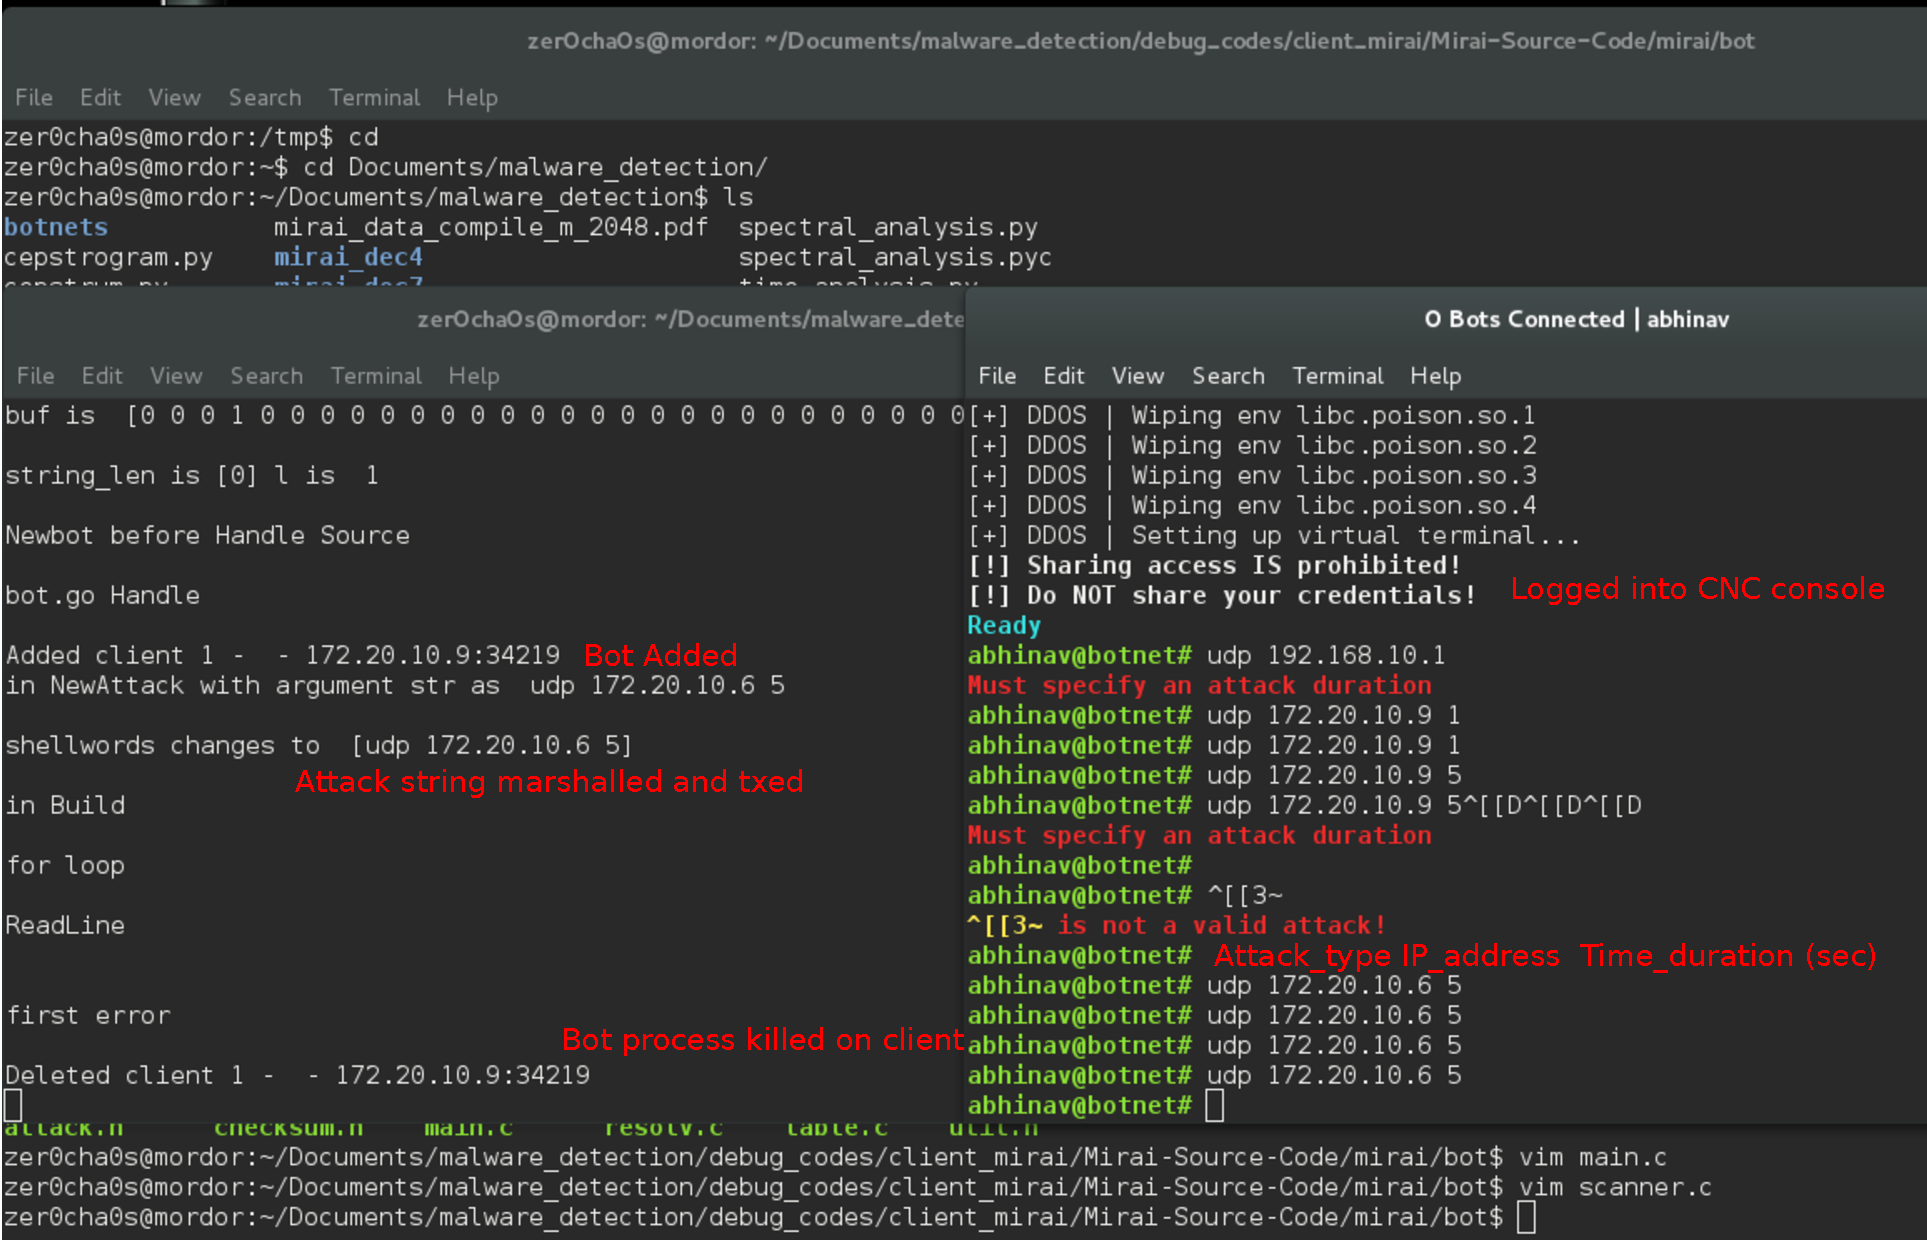
\includegraphics[width=1.3\textwidth]{mirai_attack_cnc_side.pdf}
\caption{Attack issued on CNC window. UDP flood for 5 seconds}
\label{fig:mirai_cnc_server}
\end{figure}

\begin{figure}[t!]
\centering
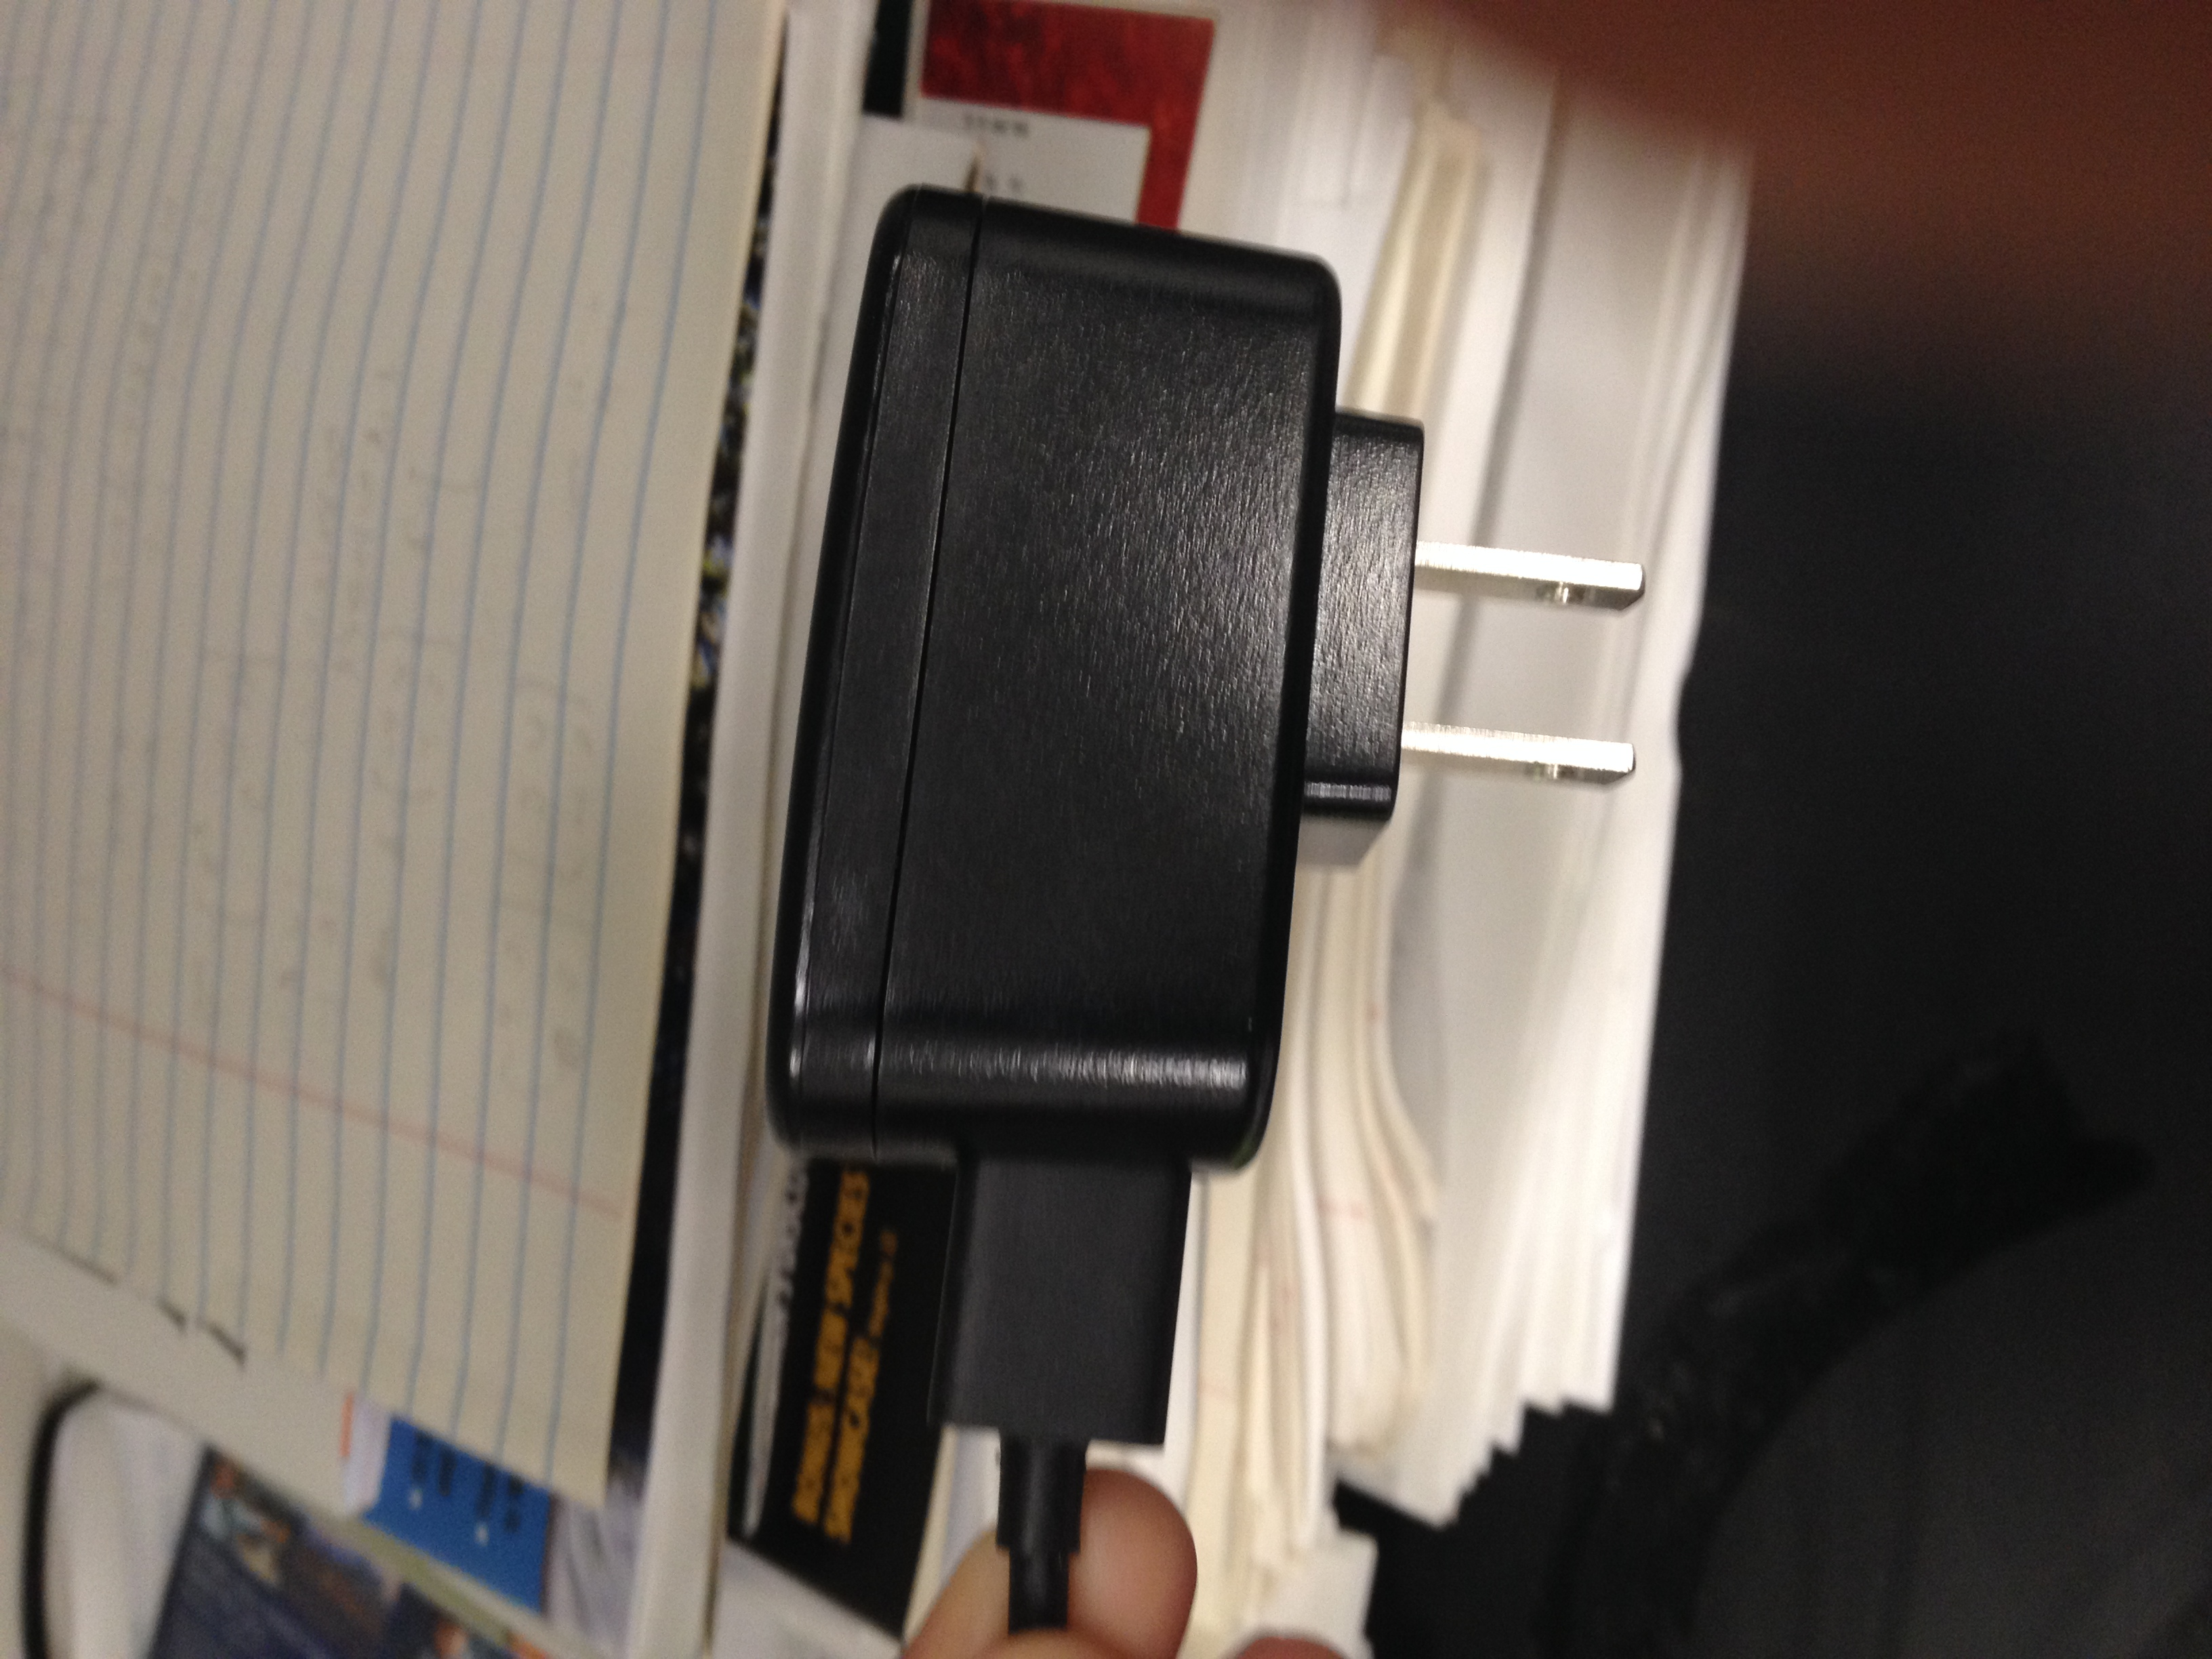
\includegraphics[width=.5\textwidth]{photo.JPG}
\caption{USB to powerline converter adapter for Raspberry Pi}
\label{fig:usb-raspi}
\end{figure}

\end{document}




